\chapter{Tyres}
\label{chap:tyres}
Tyres are the main source of external forces and moments acting upon any road vehicle\cite{milliken1995race}, for this reason, understanding their behaviour is key in making accurate predictions about vehicle dynamics. The tyre is a very complex system exhibiting high non linearities, especially in the wide operating range imposed by racing.
A realistic model of the road-vehicle interaction is clearly necessary in order to obtain significant results from simulations but the detailed study of tyres is far beyond the objectives of this work.
The present chapter provides only the fundamental concepts behind tire modelling needed to introduce the numerical model that was used.
\section{Tyre modelling basics and definitions}
\label{sec:tyrebasics}
All forces acting between the vehicle and the road are distributed over the surfaces of the so called \textit{tyre contact patches}. As the tyre contact patches size and shape are dependent on the operating conditions \cite{pac2012}, for each wheel, we consider a \textit{tyre contact point}, $C$, as the point at which an applied vector can approximate all forces acting between the tyre and the road.

The definitions used in this work are consistent with the SAE J670 standard, although simplified.

Various definitions for this point may be used to include more or less complicated effects due to tyre compliance, such as dynamic caster or centrifugal deformation.
Modelling of such phenomena would require extensive experimental data and is considered to be outside the scope of this research, thus, the following simplified definition for the tyre contact point was deemed satisfactory. The road is assumed to be a flat and planar surface and the tyre is to be considered as an infinitely thin rigid disk tangent to this plane.  The tangent point will be considered as the tyre contact point.

The wheel co-ordinate system is required for the definition of all the related physical quantities. See figure \ref{tyresystem}.
\begin{figure}[tb]
  \centering
  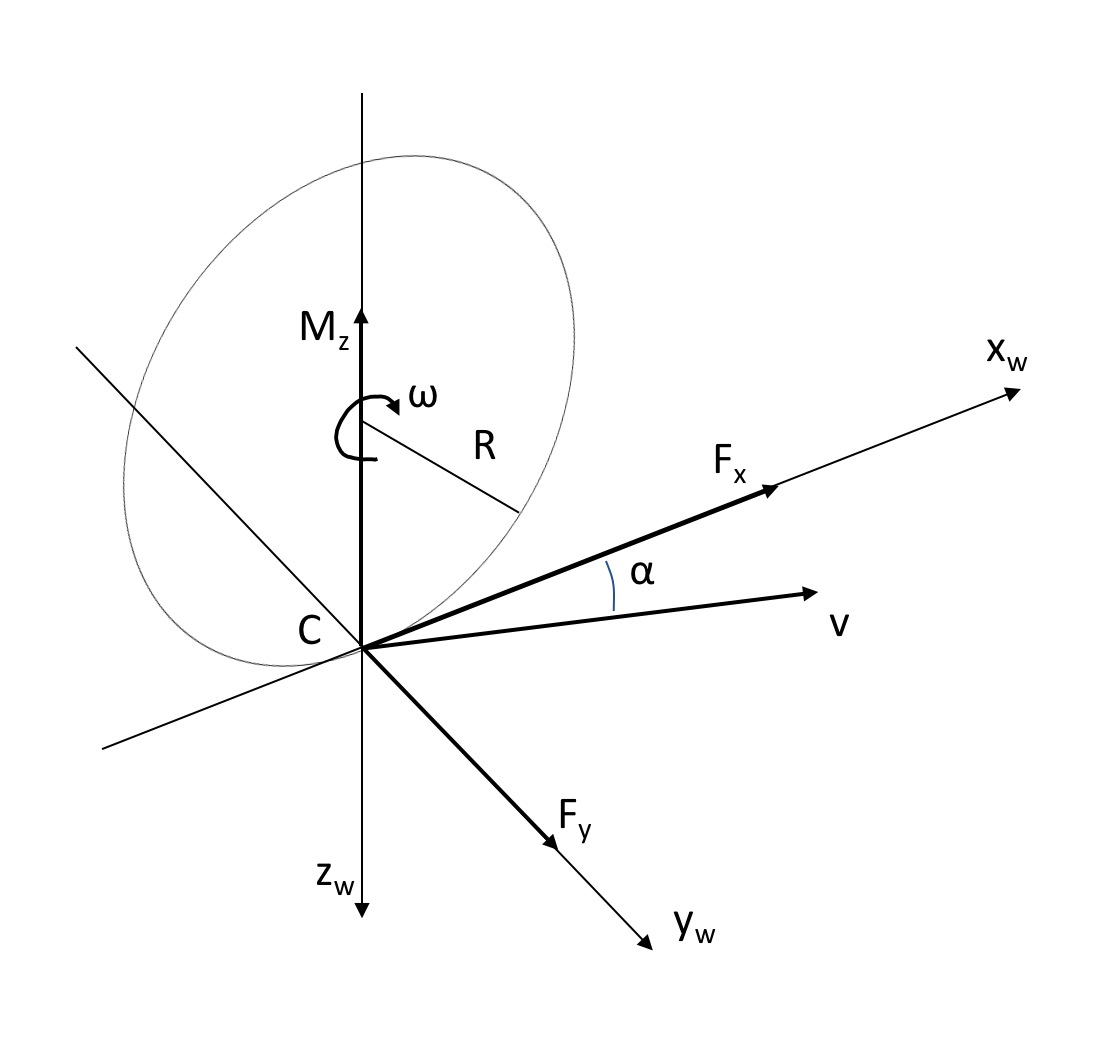
\includegraphics[height = 8cm]{images/tyresystem}
  \caption{Forces and velocities in the wheel reference system.}
  \label{tyresystem}
\end{figure}

We consider a reference system with origin in $C$, whose $x$ axis lies along the intersection between the road plane and the wheel plane, such that it is generally oriented in the direction of motion, and whose $z$ axis is pointing down, perpendicular to the road plane, the $y$ axis is determined by asserting $Cxyz$ to be a right-handed cartesian coordinate system.

The angle between the $xz$ plane and the tyre plane is known as the camber angle, it is assumed to be zero throughout this work.

The $x$, $y$ and $z$ axes are respectively associated with the \textit{longitudinal}, \textit{lateral} and \textit{vertical} dimensions of the wheel.

As tyre compliance is neglected in this work, the vertical force $F_z$ acting through the tyre and its contact point is considered as indipendent of tyre behaviour. This choice also excludes all transient responses of the rubber. The longitudinal and lateral friction forces, $F_x$ and $F_y$, are to be computed since these are what effectively make the vehicle accelerate and corner and are of primary interest.

Consider a wheel having radius $R$ and angular velocity $\omega$ about it's spin axis, passing through the wheel center and orthogonal to the wheel plane.
We consider $\omega$ as positive when the upper half of the wheel is moving in the positive $x$ direction. The lowest point of the wheel is then moving with velocity $v_{w} = -\omega R$ in the wheel $x$ direction.
By considering the velocity vector of the point $C$ in a road-fixed reference system and letting $v_x$ and $v_y$ be its components along the wheel $x$ and $y$ axes the longitudinal velocity of the road with respect to the wheel system is $v_{rx} = - v_x$.
It is therefore possible to define the longitudinal slip as the difference between these two velocities at the contact point:
$$v_{sx} = v_{w} - v_{rx} = v_x - \omega R .$$

We further define the slip ratio as
$$ \kappa = - \frac{v_{sx}}{v_{x}} = \frac{\omega R}{v_x}-1.$$
The slip angle $\alpha$ is the angle formed between the contact point velocity vector in the road frame and the wheel $x$ axis. It can be formally defined by the equation
$$\tan{\alpha} = \frac{v_y}{v_x}.$$

$F_x$ and $F_y$ scale almost linearly with the vertical load exerted on the tyre, for this reason it makes sense to define the longitudinal and lateral friction coefficients as
$$ \mu_x = \frac{F_x}{F_z} \quad\quad\quad \mu_y = \frac{F_y}{F_z}$$
$\kappa$ and $\alpha$ are the primary variables affecting the friction coefficients and are used to estimate $\mu_x$ and $\mu_y$. However, there are other factors that define the steady state tyre behaviour, some of which are relatively straight-forward, such as camber angle, vertical load, wheel rotational velocity, tyre pressure and temperature and others which are extremely difficult to quantify, such as asphalt characteristics and rubber aging.

The typical correlation between friction coefficient and slip ratio is shown in
figure \ref{kienckeplot}, ideally, all curves pass through the origin, due to the fact that without slip the speed of the wheel is the same as that of the contact point, and no friction forces can be generated. In reality, there is a slight offset caused by rolling resistance and asymmetric tyre contructions \cite{pac2012}.

\begin{figure}[tb]
  \centering
  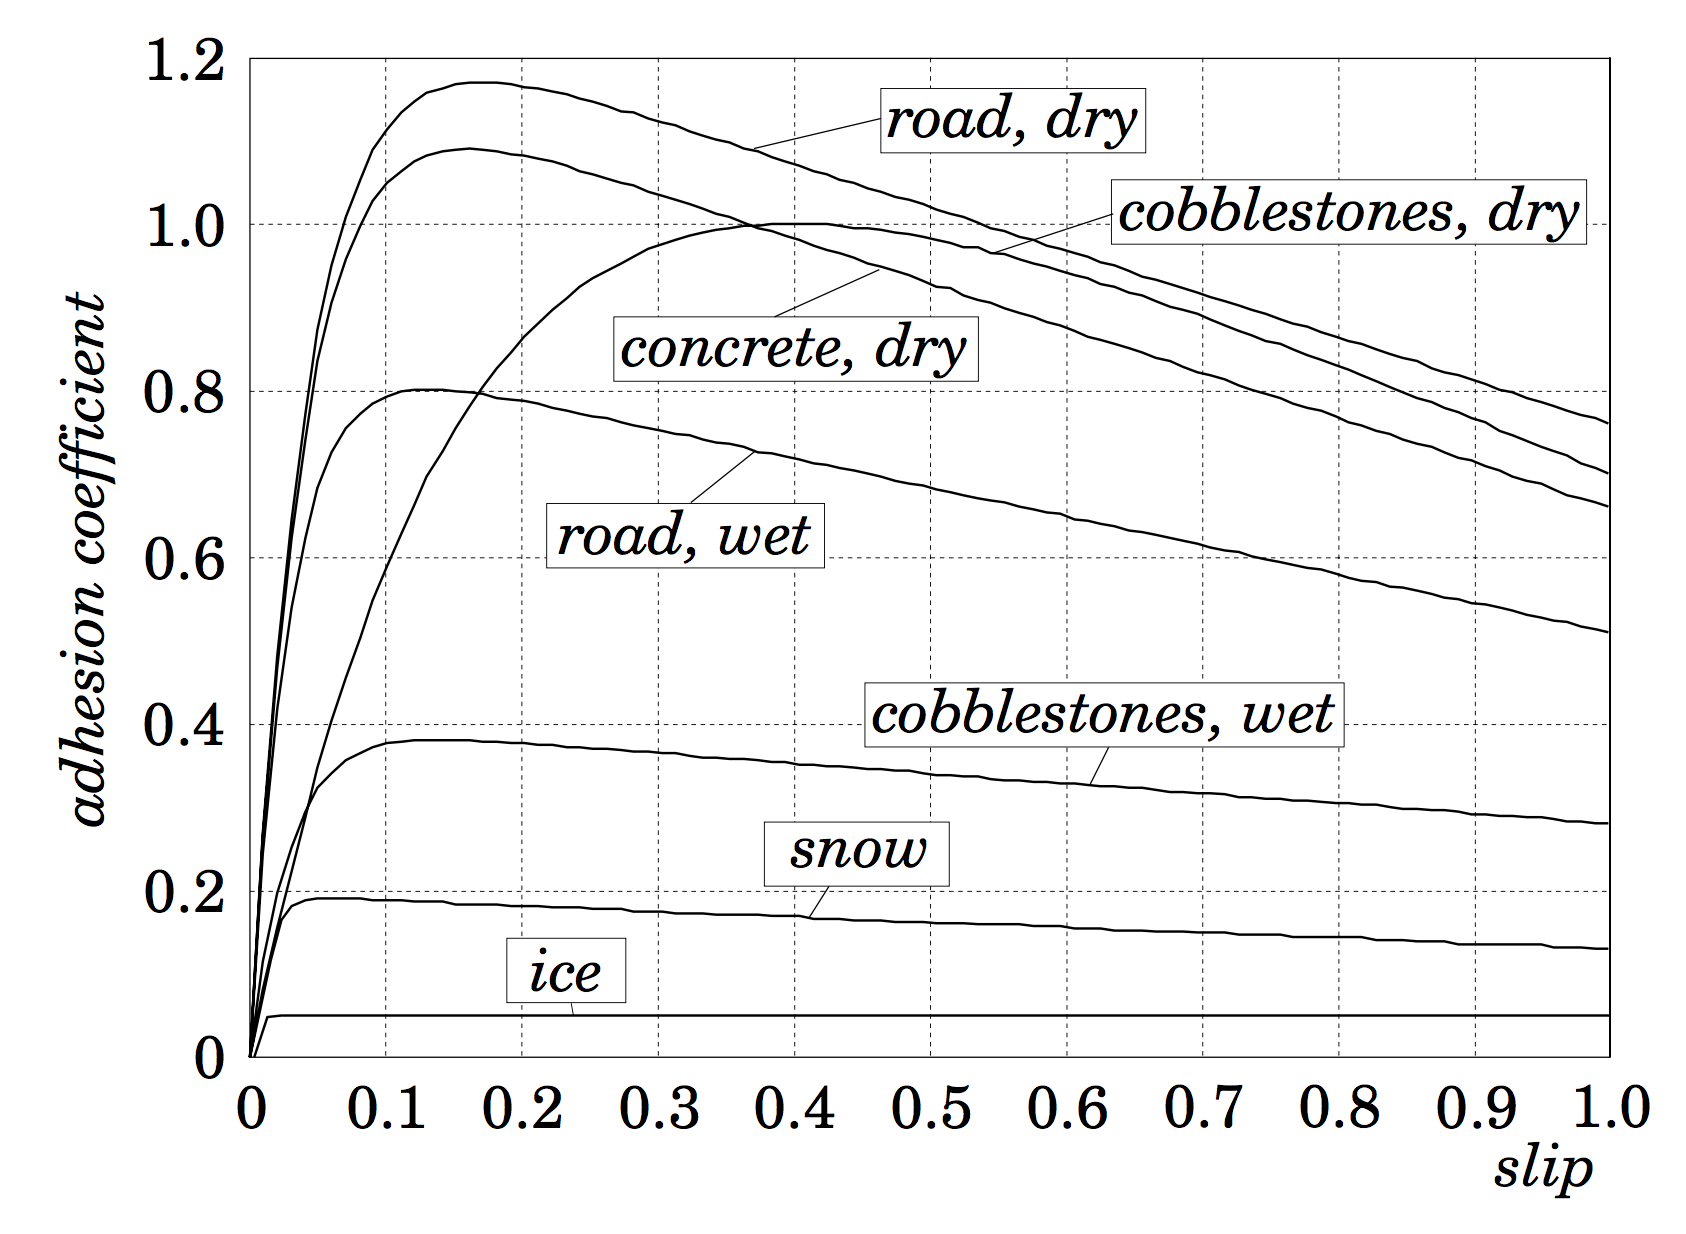
\includegraphics[height=7cm]{images/kiencke}
  \caption{Longitudinal friction coefficient under various conditions. [source: \cite{kiencke}].}
  \label{kienckeplot}
\end{figure}


It is also clearly noticeable that in order to obtain maximum longitudinal traction their will be an optimal amount of slip ratio. Limiting the tractive torque to not exceed this value is the exact purpouse of launch control systems.

Another effect of the pneumatic tyre is the so called self aligning torque, this moment is exerted about the tyre $z$ axis and is an important contributor to the steering effort which is applied to the steering wheel, this will be relevant to the steering dynamics introduced in the 12 DoF model presented in Chapter \ref{chap:12dof}.

\section{Magic Formula tyre models}
\label{sec:mf}
A series of semi-empirical tyre models was developed during the past 30 years by Hans B. Pacejka of Delft University.

These models are based on the same parametric mathematical expression, nicknamed \textit{Magic Formula} because of the good fitting properties it offers despite the lack of a physical foundation. The general form of these functions is
$$ R(k) = d\sin(c\arctan(b(1-e)k+e\arctan(bk))) $$
where $R$ is the physical quantity to be estimatated and $k$ is the most relevant variable whilst $d$, $c$, $b$, $e$ and $k$ are fitting coefficients, which may in turn depend on other variables.
The set of equations released in 1996, called \textit{Deft Tyre 96} \cite{pac96} was the first to include combined effects of longitudinal and lateral slip, subsequent editions of the model have been conceived to model tyre pressure changes \cite{pac10} and more.
The version which has been chosen in this work is the PAC2002 model \cite{pac2002}, as formalized by MSC Software and released as part of their Adams CAR multibody simulation package, which includes a set of tools for obtaining the fitting coefficients from experimental datasets. The standard file format used for the storage of the tyre coefficients is text based and can also be interpreted by an appropriate MATLAB script\cite{loadtir}.
The input variables of this tyre model are the slip ratio, slip angle, vertical force and camber angle. Outputs are the longitudinal and lateral forces and the self aligning torque.

\section{Tyre Data}
\label{sec:tyredata}

Experimental tyre data that is specific to Formula SAE and Formula Student tyres has been gathered by the FSAE Tyre Test Consortium at the Calspan test facility. The expensive tests are funded by the one-time fee the student teams pay to access the information.
As access to experimental data was not possible during the preparation of this work, a sample tyre model was used. As the coefficients were given, the fitting process was not necessary.
To verify that the tyre model was consistent with the physical intuitions developed so far, some plots were drawn (shown in figure \ref{tyreplots}), these both exhibit a plausible correlation between the slip quantities and the friction forces.

\begin{figure}[ht]
  \centering
  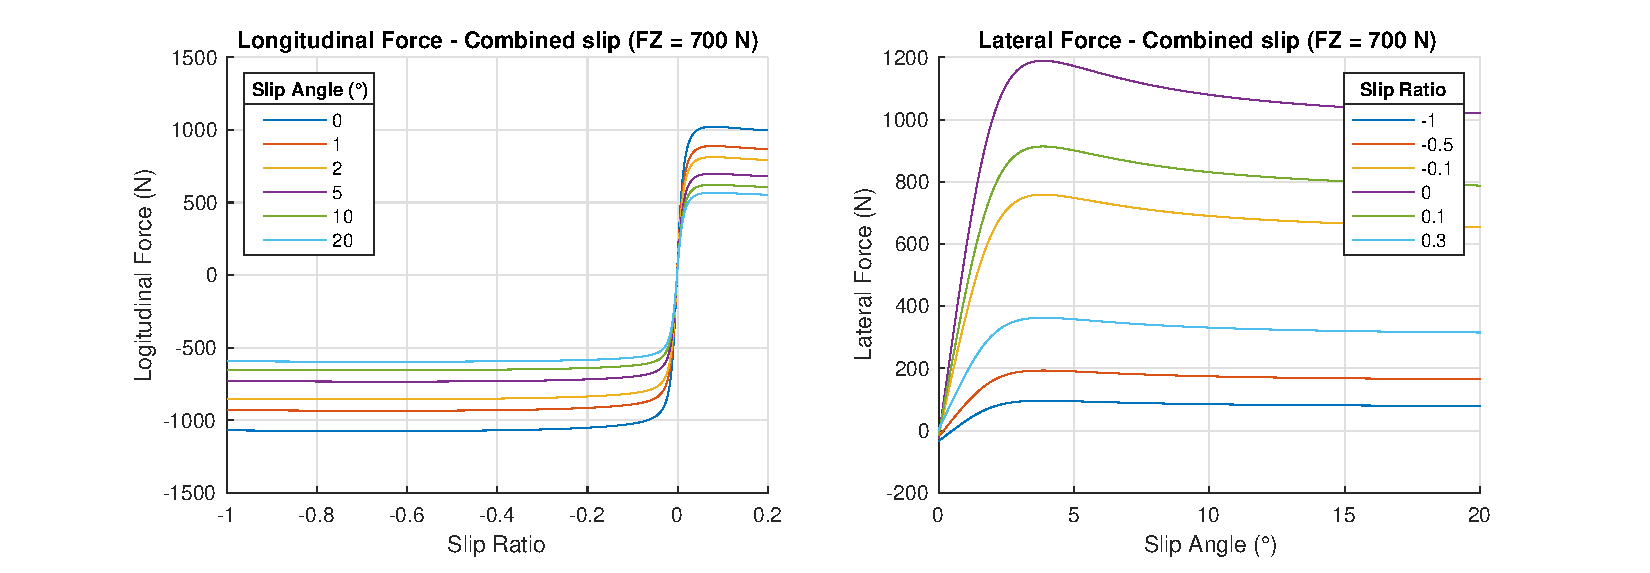
\includegraphics[width=\textwidth]{figures/tyremodel}
  \caption{Longitudinal and Lateral forces in various combined slip conditions.}
  \label{tyreplots}
\end{figure}
